\documentclass[twoside]{book}

% Packages required by doxygen
\usepackage{calc}
\usepackage{doxygen}
\usepackage{graphicx}
\usepackage[utf8]{inputenc}
\usepackage{makeidx}
\usepackage{multicol}
\usepackage{multirow}
\usepackage{fixltx2e}
\PassOptionsToPackage{warn}{textcomp}
\usepackage{textcomp}
\usepackage[nointegrals]{wasysym}
\usepackage[table]{xcolor}

% Font selection
\usepackage[T1]{fontenc}
\usepackage{mathptmx}
\usepackage[scaled=.90]{helvet}
\usepackage{courier}
\usepackage{amssymb}
\usepackage{sectsty}
\renewcommand{\familydefault}{\sfdefault}
\allsectionsfont{%
  \fontseries{bc}\selectfont%
  \color{darkgray}%
}
\renewcommand{\DoxyLabelFont}{%
  \fontseries{bc}\selectfont%
  \color{darkgray}%
}
\newcommand{\+}{\discretionary{\mbox{\scriptsize$\hookleftarrow$}}{}{}}

% Page & text layout
\usepackage{geometry}
\geometry{%
  a4paper,%
  top=2.5cm,%
  bottom=2.5cm,%
  left=2.5cm,%
  right=2.5cm%
}
\tolerance=750
\hfuzz=15pt
\hbadness=750
\setlength{\emergencystretch}{15pt}
\setlength{\parindent}{0cm}
\setlength{\parskip}{0.2cm}
\makeatletter
\renewcommand{\paragraph}{%
  \@startsection{paragraph}{4}{0ex}{-1.0ex}{1.0ex}{%
    \normalfont\normalsize\bfseries\SS@parafont%
  }%
}
\renewcommand{\subparagraph}{%
  \@startsection{subparagraph}{5}{0ex}{-1.0ex}{1.0ex}{%
    \normalfont\normalsize\bfseries\SS@subparafont%
  }%
}
\makeatother

% Headers & footers
\usepackage{fancyhdr}
\pagestyle{fancyplain}
\fancyhead[LE]{\fancyplain{}{\bfseries\thepage}}
\fancyhead[CE]{\fancyplain{}{}}
\fancyhead[RE]{\fancyplain{}{\bfseries\leftmark}}
\fancyhead[LO]{\fancyplain{}{\bfseries\rightmark}}
\fancyhead[CO]{\fancyplain{}{}}
\fancyhead[RO]{\fancyplain{}{\bfseries\thepage}}
\fancyfoot[LE]{\fancyplain{}{}}
\fancyfoot[CE]{\fancyplain{}{}}
\fancyfoot[RE]{\fancyplain{}{\bfseries\scriptsize Generated on Mon Nov 17 2014 14\+:02\+:42 for Sudoku by Doxygen }}
\fancyfoot[LO]{\fancyplain{}{\bfseries\scriptsize Generated on Mon Nov 17 2014 14\+:02\+:42 for Sudoku by Doxygen }}
\fancyfoot[CO]{\fancyplain{}{}}
\fancyfoot[RO]{\fancyplain{}{}}
\renewcommand{\footrulewidth}{0.4pt}
\renewcommand{\chaptermark}[1]{%
  \markboth{#1}{}%
}
\renewcommand{\sectionmark}[1]{%
  \markright{\thesection\ #1}%
}

% Indices & bibliography
\usepackage{natbib}
\usepackage[titles]{tocloft}
\setcounter{tocdepth}{3}
\setcounter{secnumdepth}{5}
\makeindex

% Hyperlinks (required, but should be loaded last)
\usepackage{ifpdf}
\ifpdf
  \usepackage[pdftex,pagebackref=true]{hyperref}
\else
  \usepackage[ps2pdf,pagebackref=true]{hyperref}
\fi
\hypersetup{%
  colorlinks=true,%
  linkcolor=blue,%
  citecolor=blue,%
  unicode%
}

% Custom commands
\newcommand{\clearemptydoublepage}{%
  \newpage{\pagestyle{empty}\cleardoublepage}%
}


%===== C O N T E N T S =====

\begin{document}

% Titlepage & ToC
\hypersetup{pageanchor=false,
             bookmarks=true,
             bookmarksnumbered=true,
             pdfencoding=unicode
            }
\pagenumbering{roman}
\begin{titlepage}
\vspace*{7cm}
\begin{center}%
{\Large Sudoku }\\
\vspace*{1cm}
{\large Generated by Doxygen 1.8.7}\\
\vspace*{0.5cm}
{\small Mon Nov 17 2014 14:02:42}\\
\end{center}
\end{titlepage}
\clearemptydoublepage
\tableofcontents
\clearemptydoublepage
\pagenumbering{arabic}
\hypersetup{pageanchor=true}

%--- Begin generated contents ---
\chapter{Hierarchical Index}
\section{Class Hierarchy}
This inheritance list is sorted roughly, but not completely, alphabetically\+:\begin{DoxyCompactList}
\item \contentsline{section}{Database}{\pageref{class_database}}{}
\item Q\+Dialog\begin{DoxyCompactList}
\item \contentsline{section}{How\+To\+Dialog}{\pageref{class_how_to_dialog}}{}
\item \contentsline{section}{New\+Game}{\pageref{class_new_game}}{}
\end{DoxyCompactList}
\item Q\+Main\+Window\begin{DoxyCompactList}
\item \contentsline{section}{Game\+Window}{\pageref{class_game_window}}{}
\item \contentsline{section}{Main\+Window}{\pageref{class_main_window}}{}
\end{DoxyCompactList}
\item \contentsline{section}{Settings}{\pageref{class_settings}}{}
\end{DoxyCompactList}

\chapter{Class Index}
\section{Class List}
Here are the classes, structs, unions and interfaces with brief descriptions\+:\begin{DoxyCompactList}
\item\contentsline{section}{\hyperlink{class_database}{Database} }{\pageref{class_database}}{}
\item\contentsline{section}{\hyperlink{class_game_window}{Game\+Window} }{\pageref{class_game_window}}{}
\item\contentsline{section}{\hyperlink{class_how_to_dialog}{How\+To\+Dialog} }{\pageref{class_how_to_dialog}}{}
\item\contentsline{section}{\hyperlink{class_main_window}{Main\+Window} }{\pageref{class_main_window}}{}
\item\contentsline{section}{\hyperlink{class_new_game}{New\+Game} }{\pageref{class_new_game}}{}
\item\contentsline{section}{\hyperlink{class_settings}{Settings} }{\pageref{class_settings}}{}
\end{DoxyCompactList}

\chapter{Class Documentation}
\hypertarget{class_database}{\section{Database Class Reference}
\label{class_database}\index{Database@{Database}}
}
\subsection*{Public Member Functions}
\begin{DoxyCompactItemize}
\item 
\hypertarget{class_database_a5d8bbb846ab518f7f3972124cbb1d867}{{\bfseries Database} (Q\+String, Q\+String, Q\+String, Q\+String)}\label{class_database_a5d8bbb846ab518f7f3972124cbb1d867}

\item 
\hypertarget{class_database_a2925e696474bdfc43a46f7142e2975ea}{Q\+Sql\+Database {\bfseries get\+Db} ()}\label{class_database_a2925e696474bdfc43a46f7142e2975ea}

\item 
void \hyperlink{class_database_ac314f58ea7be59d587d60f3ece8892f9}{init} (Q\+String, Q\+String, Q\+String, Q\+String)
\begin{DoxyCompactList}\small\item\em \hyperlink{class_database_ac314f58ea7be59d587d60f3ece8892f9}{Database\+::init}. \end{DoxyCompactList}\item 
\hypertarget{class_database_a91a1c183ac9952a171aba2229e711ebd}{Q\+String {\bfseries get\+Hostname} () const }\label{class_database_a91a1c183ac9952a171aba2229e711ebd}

\item 
\hypertarget{class_database_ae1108262c8940e898d85d132f79c4441}{void {\bfseries set\+Hostname} (const Q\+String \&value)}\label{class_database_ae1108262c8940e898d85d132f79c4441}

\item 
\hypertarget{class_database_a06ad7206bbd4bd4d5bae07d45f741e29}{Q\+String {\bfseries get\+User} () const }\label{class_database_a06ad7206bbd4bd4d5bae07d45f741e29}

\item 
\hypertarget{class_database_a8208ef97013e8c36323374f05214e3ed}{void {\bfseries set\+User} (const Q\+String \&value)}\label{class_database_a8208ef97013e8c36323374f05214e3ed}

\item 
\hypertarget{class_database_ac3c422af93ce292c2500ee55ded5a8ff}{Q\+String {\bfseries get\+Password} () const }\label{class_database_ac3c422af93ce292c2500ee55ded5a8ff}

\item 
\hypertarget{class_database_a832022d7c4c640e04f253c7961ca6547}{void {\bfseries set\+Password} (const Q\+String \&value)}\label{class_database_a832022d7c4c640e04f253c7961ca6547}

\item 
\hypertarget{class_database_a86a3478674801832b0cf05aa41193820}{Q\+String {\bfseries get\+Db\+Name} () const }\label{class_database_a86a3478674801832b0cf05aa41193820}

\item 
\hypertarget{class_database_a5d0c6de89689f4f8ad6500969031dfd0}{void {\bfseries set\+Db\+Name} (const Q\+String \&value)}\label{class_database_a5d0c6de89689f4f8ad6500969031dfd0}

\end{DoxyCompactItemize}


\subsection{Member Function Documentation}
\hypertarget{class_database_ac314f58ea7be59d587d60f3ece8892f9}{\index{Database@{Database}!init@{init}}
\index{init@{init}!Database@{Database}}
\subsubsection[{init}]{\setlength{\rightskip}{0pt plus 5cm}void Database\+::init (
\begin{DoxyParamCaption}
\item[{Q\+String}]{host, }
\item[{Q\+String}]{db\+Name, }
\item[{Q\+String}]{user, }
\item[{Q\+String}]{pass}
\end{DoxyParamCaption}
)}}\label{class_database_ac314f58ea7be59d587d60f3ece8892f9}


\hyperlink{class_database_ac314f58ea7be59d587d60f3ece8892f9}{Database\+::init}. 

sets all the values also basically a bug fix 
\begin{DoxyParams}{Parameters}
{\em host} & \\
\hline
{\em db\+Name} & \\
\hline
{\em user} & \\
\hline
{\em pass} & \\
\hline
\end{DoxyParams}


The documentation for this class was generated from the following files\+:\begin{DoxyCompactItemize}
\item 
database.\+h\item 
database.\+cpp\end{DoxyCompactItemize}

\hypertarget{class_game_window}{\section{Game\+Window Class Reference}
\label{class_game_window}\index{Game\+Window@{Game\+Window}}
}
Inheritance diagram for Game\+Window\+:\begin{figure}[H]
\begin{center}
\leavevmode
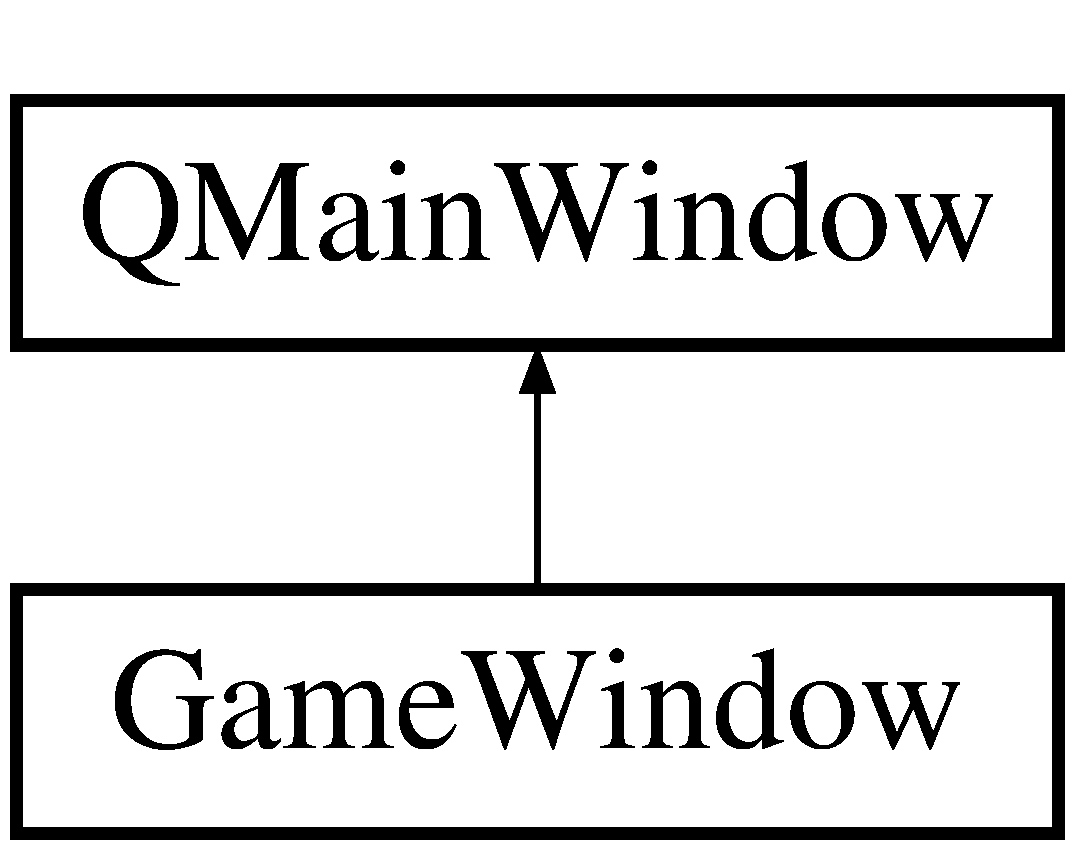
\includegraphics[height=2.000000cm]{class_game_window}
\end{center}
\end{figure}
\subsection*{Public Member Functions}
\begin{DoxyCompactItemize}
\item 
\hypertarget{class_game_window_a66368faf09314c3d4c30c9853de8fb20}{{\bfseries Game\+Window} (Q\+Widget $\ast$parent=0, int level=0)}\label{class_game_window_a66368faf09314c3d4c30c9853de8fb20}

\end{DoxyCompactItemize}


The documentation for this class was generated from the following files\+:\begin{DoxyCompactItemize}
\item 
gamewindow.\+h\item 
gamewindow.\+cpp\end{DoxyCompactItemize}

\hypertarget{class_how_to_dialog}{\section{How\+To\+Dialog Class Reference}
\label{class_how_to_dialog}\index{How\+To\+Dialog@{How\+To\+Dialog}}
}


Inheritance diagram for How\+To\+Dialog\+:


Collaboration diagram for How\+To\+Dialog\+:
\subsection*{Public Member Functions}
\begin{DoxyCompactItemize}
\item 
\hypertarget{class_how_to_dialog_ae1cee44a39ca4f51994de2e4067e6121}{{\bfseries How\+To\+Dialog} (Q\+Widget $\ast$parent=0)}\label{class_how_to_dialog_ae1cee44a39ca4f51994de2e4067e6121}

\end{DoxyCompactItemize}


The documentation for this class was generated from the following files\+:\begin{DoxyCompactItemize}
\item 
howtodialog.\+h\item 
howtodialog.\+cpp\end{DoxyCompactItemize}

\hypertarget{class_main_window}{\section{Main\+Window Class Reference}
\label{class_main_window}\index{Main\+Window@{Main\+Window}}
}
Inheritance diagram for Main\+Window\+:\begin{figure}[H]
\begin{center}
\leavevmode
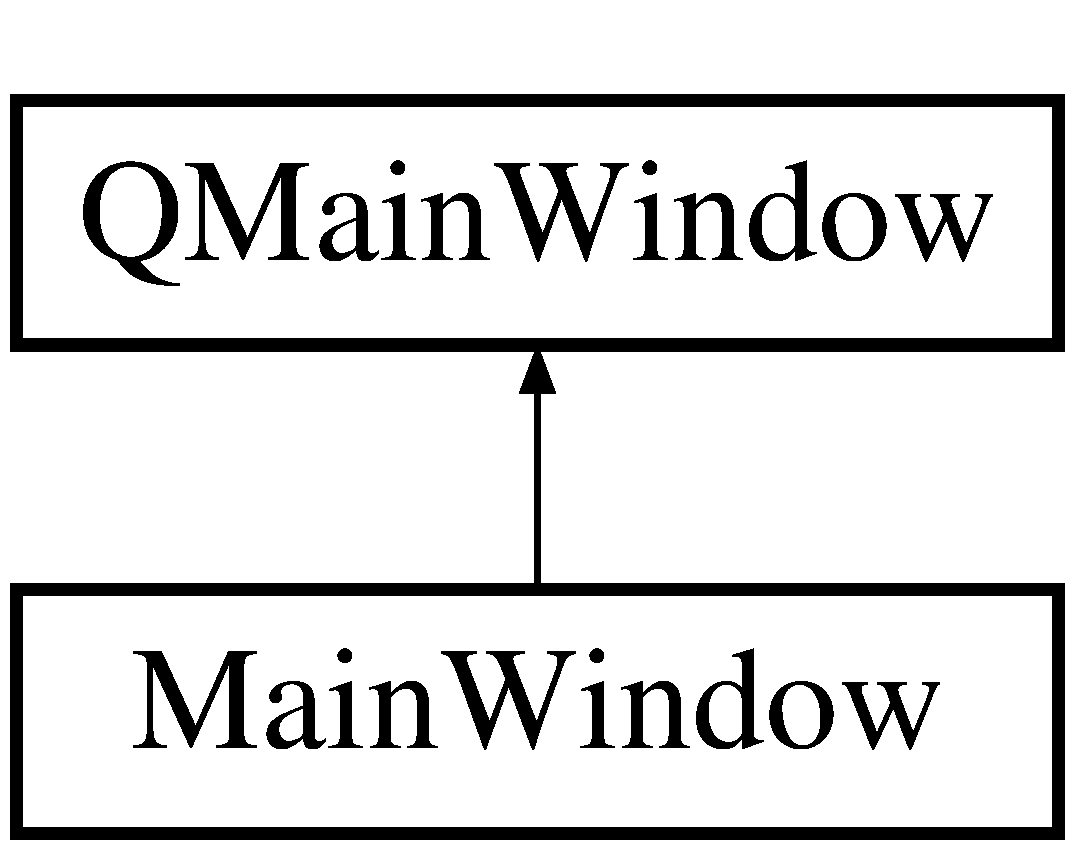
\includegraphics[height=2.000000cm]{class_main_window}
\end{center}
\end{figure}
\subsection*{Public Member Functions}
\begin{DoxyCompactItemize}
\item 
\hypertarget{class_main_window_a8b244be8b7b7db1b08de2a2acb9409db}{{\bfseries Main\+Window} (Q\+Widget $\ast$parent=0)}\label{class_main_window_a8b244be8b7b7db1b08de2a2acb9409db}

\end{DoxyCompactItemize}


The documentation for this class was generated from the following files\+:\begin{DoxyCompactItemize}
\item 
mainwindow.\+h\item 
mainwindow.\+cpp\end{DoxyCompactItemize}

\hypertarget{class_new_game}{\section{New\+Game Class Reference}
\label{class_new_game}\index{New\+Game@{New\+Game}}
}
Inheritance diagram for New\+Game\+:\begin{figure}[H]
\begin{center}
\leavevmode
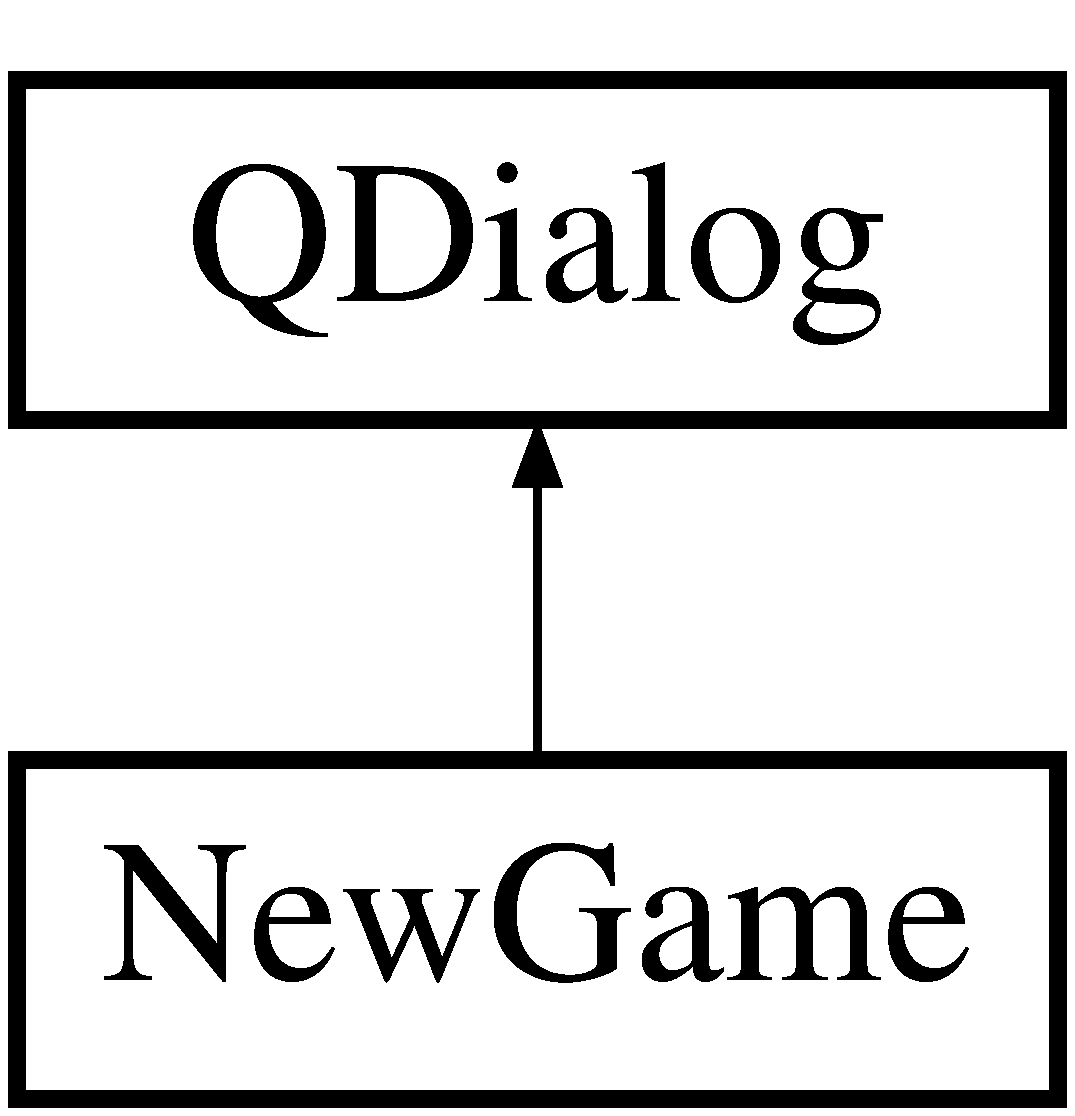
\includegraphics[height=2.000000cm]{class_new_game}
\end{center}
\end{figure}
\subsection*{Public Member Functions}
\begin{DoxyCompactItemize}
\item 
\hypertarget{class_new_game_abc0dccbe2a43eef32570473265de9a8a}{{\bfseries New\+Game} (Q\+Widget $\ast$parent=0)}\label{class_new_game_abc0dccbe2a43eef32570473265de9a8a}

\end{DoxyCompactItemize}


The documentation for this class was generated from the following file\+:\begin{DoxyCompactItemize}
\item 
newgame.\+h\end{DoxyCompactItemize}

%--- End generated contents ---

% Index
\newpage
\phantomsection
\addcontentsline{toc}{chapter}{Index}
\printindex

\end{document}
